\subsection{Comparison of the approaches} \label{results_final}

\begin{figure}
  \begin{subfigure}[t]{.32\textwidth}
    \centering
    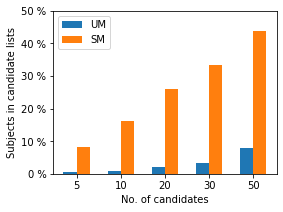
\includegraphics[width=\textwidth]{figures/supervised_approach/compare_hw.png}
    \caption{Handwritten subjects}
    \label{fig:compare_hw}
  \end{subfigure}
  \begin{subfigure}[t]{.32\textwidth}
    \centering
    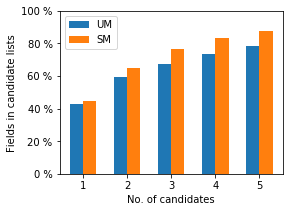
\includegraphics[width=\textwidth]{figures/supervised_approach/compare_ddc.png}
    \caption{DDC subjects}
    \label{fig:compare_ddc}
  \end{subfigure}
   \begin{subfigure}[t]{.32\textwidth}
    \centering
    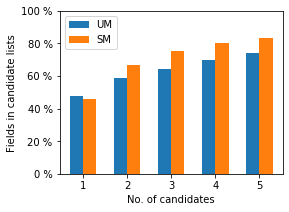
\includegraphics[width=\textwidth]{figures/supervised_approach/compare_venue.png}
    \caption{Venues}
    \label{fig:compare_venue}
  \end{subfigure}
  \caption{Hit rate of the approaches for the evaluation sets.}
  \label{fig:compare_eval}
\end{figure}

\begin{figure}
    \centering
    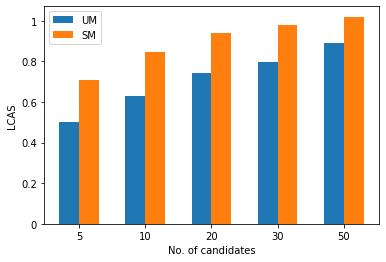
\includegraphics[width=.6\textwidth]{figures/evaluation/compare_lcas.png}
    \caption{LCAS comparison of the approaches.}
    \label{fig:compare_lcas}
\end{figure}

In this section, we compare the unsupervised approach with the best performing supervised model, i.e. the \acrshort{bce} model. We refer to them as \acrfull{um} and \acrfull{sm}, respectively. The \acrshort{sm} outperforms the \acrshort{um} in all evaluation sets, as shown in figure \ref{fig:compare_eval}. The \acrshort{sm} is better at identifying fields than the \acrshort{um}. It performs consistently better on the \acrshort{ddc} and venue evaluation sets. However, the difference in hit rate is the largest for the handwritten set.

Only in the venue set for one candidate does the \acrshort{um} perform better, by a margin of 2 \%. For all other number of candidates, the \acrshort{sm} performs better, by a margin from 8 to 11 \%. The differences on the \acrshort{ddc} set are similar. The difference in performance when identifying all 2,157 subjects is much larger, also in favor of the \acrshort{sm}. The difference between them goes from 8 \% when 5 candidates are considered, to 36 \% for 50 candidates.

The superiority of the \acrshort{sm} on the handwritten set is also confirmed by the \acrshort{lcas}, shown in figure \ref{fig:compare_lcas}. Given the large difference in hit rate between the models, this result is to be expected. However, that the \acrshort{lcas} difference is smaller than the difference in hit rate indicates that the guesses of the \acrshort{um} are close to the correct subjects. This hypothesis is also supported by the high hit rate of the \acrshort{um} when identifying fields in the other two evaluation sets.